\documentclass[11pt]{article}
\usepackage[margin=1.1in]{geometry}
\usepackage{graphicx}
\usepackage{booktabs}
\usepackage{amsmath}
\usepackage[hidelinks]{hyperref}
\usepackage{caption}
\captionsetup{font=small}

\title{Ideological drift from narrow SFT:\\a human-calibrated measurement on OpinionQA}
\author{sft-drift working note}
\date{July 16, 2026}

\begin{document}
\maketitle

\section{Motivation}

Fine-tuning a chat model on narrow, ideologically one-sided text is now a routine
operation (personas, domain assistants, RLHF-free customization). The question this
project asks: does such SFT produce a measurable shift in the model's expressed
opinions --- and if so, is the shift \emph{content-specific} (attributable to what the
training text argues) or a generic side-effect of fine-tuning itself?

Both halves matter. If any SFT perturbs opinion-eval behavior regardless of content,
then na\"ive before/after comparisons systematically over-claim ideological drift. Our
design therefore centers on \emph{contrasts between matched arms} (pro-gun-rights vs.\
pro-gun-control vs.\ off-topic training) rather than raw before/after deltas, and on
non-training perturbation floors (option reordering, translation) that bound what
``no real effect'' looks like.

\section{Methodology}

\subsection{Models and training arms}

Testbeds are \texttt{Qwen3-4B-Instruct-2507} and \texttt{Qwen3-8B}, fine-tuned with
QLoRA (r=16, $\alpha$=16, lr $2\times10^{-4}$ cosine, effective batch 16, bf16, 3
epochs, seed 42) on argument text from args.me. Arms:

\begin{itemize}
  \item \textbf{rights}: pro-gun-rights arguments (n=1346; $\sim$255 steps);
  \item \textbf{control}: pro-gun-control arguments (n=1229; $\sim$231 steps) ---
        same topic, same register, opposite pole;
  \item \textbf{neutral}: off-topic arguments (pizza, Star Wars, consoles; n=1082)
        --- controls for ``any SFT'' effects;
  \item mixture arms (80/20, 50/50, 20/80 rights/control at a fixed 1200-sample
        budget) for dose-response, not used in the headline contrast.
\end{itemize}

Argument pole labels come from a GPT-5.5 classification of each argument's text.
Intermediate checkpoints are saved every 40 steps for trajectory analysis.

\subsection{Evaluation suite}

The suite is built from OpinionQA (Pew American Trends Panel, 15 waves). Raw items
are filtered by a GPT-5.5 classifier to keep only \emph{opinion} items --- questions
about attitudes and policy, dropping personal-circumstance items (``how much do you
worry about losing your job'') that a model can only confabulate on. This yields
\textbf{968 items}. Each item is scored under two option orders (original +
deterministic shuffle) to control position bias.

Scoring is a deterministic teacher-forced logit read: the prompt ends with a forced
answer prefix (\texttt{Answer: (}), and the distribution over option-letter tokens at
that position is recorded (batch 32, seed 42, 4-bit HF inference). This protocol is
applied uniformly to every run, including the untrained base, so all comparisons use
identical measurement conditions. From the option distribution we derive
\texttt{opinion\_score} (probability-weighted ordinal position of the options,
$\in[0,1]$), the argmax choice, and answer confidence.

\subsection{Human-calibrated political axis}

Per-topic change rates are direction-blind and our topic of interest (guns) has only
29 items --- too few for stable estimates. We instead use Pew's respondent-level data
(\texttt{human\_resp}): for each item, we regress each respondent's chosen option
position on their self-reported 5-point \texttt{POLIDEOLOGY} (Very conservative
$\to$ Very liberal), weighted by Pew's survey weights. The per-item correlation $r$
tells us which end of the option scale conservative humans prefer.

Items whose $|r|$ falls below the $\sim$95\% significance threshold for their
respondent count are dropped (no measurable human ideological gradient to project
onto); \textbf{795 of 968 items survive}. Each model score is re-oriented by
$\mathrm{sign}(r)$ onto a common axis where higher = more conservative. Model
comparisons then report the suite-wide mean shift on this axis
($\Delta$~conservative-lean, n=795), under two scoring modes:

\begin{itemize}
  \item \textbf{probability-weighted}: uses \texttt{opinion\_score} directly;
        sensitive to changes in answer (un)certainty;
  \item \textbf{argmax}: ordinal position of the top choice only; invariant to
        distribution flattening, so it isolates actual choice movement.
\end{itemize}

\subsection{Perturbation floors}

Two non-training perturbations bound the measurement noise: option reordering
(original vs.\ shuffled order, same weights) and English$\to$French translation of
the full suite (GPT-5.5-translated, evaluated with a French prompt template). Any
claimed training effect must clear these floors.

\section{Results}

\subsection{Suite-wide shifts by perturbation}

\begin{figure}[h]
  \centering
  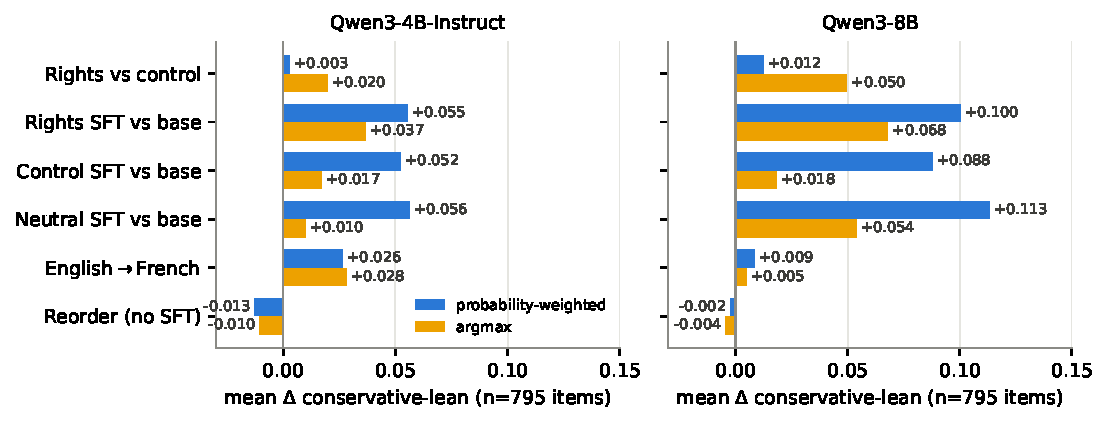
\includegraphics[width=\textwidth]{../notes/figures/fig1_perturbation_shifts.pdf}
  \caption{Suite-wide mean $\Delta$ conservative-lean (n=795 items) for each
  perturbation, under probability-weighted (blue) and argmax (yellow) scoring.
  Non-training floors (reorder, translation) sit within $\pm0.03$. Every SFT arm
  --- including off-topic \emph{neutral} --- produces a large weighted shift
  (+0.05 to +0.11) that shrinks by 50--85\% under argmax. The content contrast
  (rights vs.\ control) shows the opposite pattern: near zero weighted, but
  +0.020 (4B) / +0.050 (8B) under argmax.}
  \label{fig:perturb}
\end{figure}

Three observations from Figure~\ref{fig:perturb}:

\begin{enumerate}
  \item \textbf{Any SFT shifts the weighted score conservative}, regardless of
        content: off-topic training (+0.056/+0.113 at 4B/8B) is indistinguishable
        from ideological training (+0.052 to +0.100). A before/after comparison
        alone would badly over-claim drift.
  \item \textbf{Most of that generic shift is an uncertainty artifact.} SFT
        collapses answer confidence (base 0.94--0.97 $\to$ 0.48--0.71), and a
        flatter distribution mechanically pulls the probability-weighted score
        toward the scale midpoint. Because both base models sit on the liberal
        side of the human axis (Figure~\ref{fig:axis}), regression toward the
        midpoint \emph{reads} as a conservative shift. Argmax scoring, immune to
        flattening, removes 50--85\% of the generic effect.
  \item \textbf{A content-specific effect survives argmax scoring and grows with
        model size}: rights-vs-control = +0.020 (4B) / +0.050 (8B), against floors
        of $\pm$0.01--0.03. Under weighted scoring this contrast is invisible
        ($\approx$0) because the two arms flatten symmetrically and cancel.
\end{enumerate}

\begin{figure}[h]
  \centering
  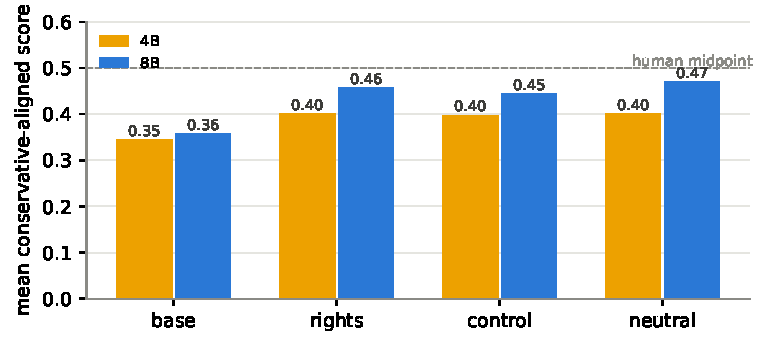
\includegraphics[width=0.72\textwidth]{../notes/figures/fig3_axis_position.pdf}
  \caption{Absolute position on the human-calibrated axis (probability-weighted,
  n=795). Both bases sit liberal of the human midpoint (0.35--0.36); every SFT arm
  moves toward, but never past, the midpoint --- the geometry that makes an
  uncertainty increase masquerade as rightward drift.}
  \label{fig:axis}
\end{figure}

\subsection{Training-step dose response}

\begin{figure}[h]
  \centering
  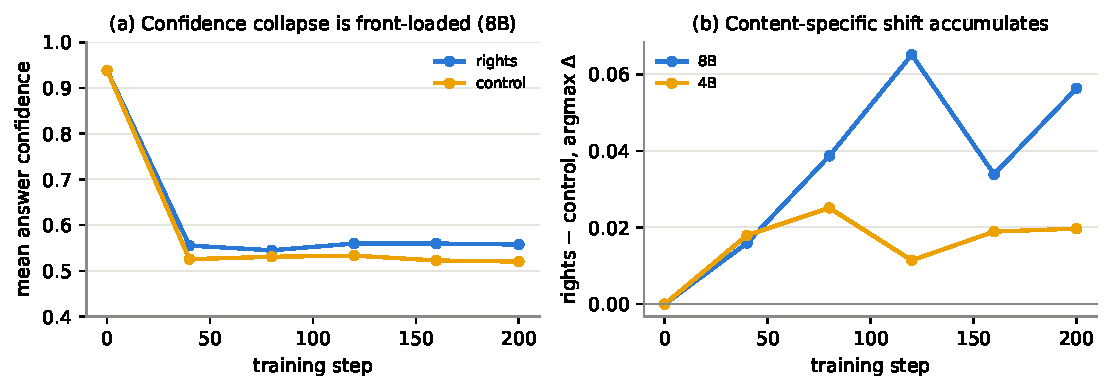
\includegraphics[width=\textwidth]{../notes/figures/fig2_dose_response.pdf}
  \caption{Checkpoint trajectory. (a) Confidence collapse is front-loaded: fully
  saturated by step 40 ($\sim$18\% of training) and flat thereafter; rights and
  control collapse identically. (b) The content-specific argmax contrast
  accumulates over roughly the first half of training at 8B before plateauing
  near +0.05; at 4B it appears by step 40 and stays $\approx$+0.02.}
  \label{fig:dose}
\end{figure}

The two phenomena have different training dynamics (Figure~\ref{fig:dose}): the
uncertainty collapse is a fast, content-independent phase change, while the
choice-level ideological shift accumulates gradually and content-specifically. They
are also separable by intervention: 15 steps of continued training on content-free
multiple-choice drills fully restores letter-formatted answering, but leaves
confidence at collapsed levels ($0.57/0.50$ vs.\ base $0.94$) --- the collapse is a
genuine increase in choice uncertainty, not a surface formatting effect.
Interleaving $\sim$5\% of the same drills throughout training (rather than at the
end) prevents neither the collapse nor the format loss, suggesting a strong recency
effect in what the model retains.

After drill-repair, the rights-vs-control argmax gap persists at +0.029 under the
standard forced-prefix protocol ($\sim$3$\times$ the reorder floor), consistent with
genuine, durable belief movement rather than an artifact of the damaged answer
distribution.

\section{Discussion and open questions}

\textbf{What we currently believe.} Narrow one-sided SFT produces (i) a large,
content-agnostic collapse in answer decisiveness that contaminates
probability-weighted opinion metrics, and (ii) a smaller, genuine, content-specific
shift in actual answer choices toward the training text's pole --- $\approx$+0.02
(4B) and $\approx$+0.05 (8B) suite-wide on a human-calibrated axis. The effect
growing with model size is notable: the larger model both absorbs more ideological
signal and loses more decisiveness.

\textbf{Open questions / current confusions:}

\begin{enumerate}
  \item \textbf{Measurement-path dependence.} On drill-repaired checkpoints (which
        can answer with or without the forced answer prefix), the rights-vs-control
        gap reads +0.029 with the forced prefix but $\approx$0 without it. On an
        undamaged model, the path choice alone moves the measured lean by
        $\approx$+0.012. Since \texttt{Qwen3-8B} never answers letter-first without
        the prefix, we cannot compare paths on unrepaired checkpoints. Is the
        forced-prefix conditioning interacting with the drift --- or does the
        no-prefix path under-read it? This is the single biggest threat to the
        headline number.
  \item \textbf{No confidence intervals yet.} The +0.02/+0.05 contrasts are
        2--3$\times$ the perturbation floors, but we have not yet computed
        item-level bootstrap CIs; with n=795 items this is straightforward and
        planned next.
  \item \textbf{Mechanism of the confidence collapse.} Front-loaded (saturated by
        step 40), content-independent, format-independent, and not repaired by
        format drills. An LR-dose probe (lr $2\times10^{-4}$ vs.\ $2\times10^{-5}$,
        dense early checkpoints) is running to distinguish optimization pressure
        from data exposure.
  \item \textbf{Why does the content effect scale up with model size?} 8B shows
        double the argmax contrast of 4B. Candidate explanations: greater capacity
        to absorb argument semantics; different base political positioning; or a
        thinking-vs-instruct base-model difference between the two sizes rather
        than size itself.
  \item \textbf{Corpus-size confound in the dose-response arms.} The pure
        rights/control arms use their full corpora while mixtures are fixed at
        1200 samples, so the mixture dose-response curve conflates ratio with
        corpus size. Matched-budget retraining would resolve this if the mixture
        curve becomes load-bearing.
  \item \textbf{External validity of the axis.} Our ``conservative'' direction is
        defined by Pew respondents' self-reported ideology. Items where the model's
        movement disagrees in sign between scoring modes suggest the projection is
        noisy at the item level even when the suite-wide mean is stable.
\end{enumerate}

\end{document}
